\section{Transposition Models, Real Geometry, and Equal-Copper Comparisons}
\label{chapter:05}

% block-id: 05.geometry.heading
\hypertarget{05.geometry.heading}{}
\subsection{Geometry sampling and discrete transposition}

% block-id: 05.geometry.p1
\hypertarget{05.geometry.p1}{}
Fig.~\ref{fig:geometry_comparison} shows straight, single-level, traditional multilevel and cross-layer centerlines. The geometry records preserve strand identity, periodicity, clearance, curvature, actual arc length and copper volume. Axial sampling at 400, 800 and 1600 points and 60 checks support sampling consistency for these quantities. The illustrated 24-strand structure with a copper diameter of 0.100 mm has a nominal copper area of approximately 0.1885 mm² and demonstrates geometry construction. A structure meeting the minimum 5 mm² copper area requires separate construction and verification. Three-dimensional views reveal spatial paths; the corresponding field-circuit model evaluates electromagnetic performance.

% block-id: 05.geometry.p2
\hypertarget{05.geometry.p2}{}
The current DTM/iDTM demonstration uses the additive discrete blocks in \eqref{eq:E06}. For the same weighted impedance blocks, their sum is invariant to ordering; this implementation therefore checks identity mappings and circuit accumulation of the specified blocks. Comparing actual transposition paths additionally requires longitudinal position changes, noncommuting relationships between levels, local fields, and terminal conditions. These assumptions determine comparability with the literature \cite{P01,N01}.

% block-id: 05.dtm_derivation.heading
\hypertarget{05.dtm_derivation.heading}{}
\subsection{Mapping strand identity to cross-sectional position}

% block-id: 05.dtm_derivation.p1
\hypertarget{05.dtm_derivation.p1}{}
Let Ps map fixed physical strand identities to spatial positions in cross-section s. Local currents are Ps i, and local voltages transformed back to identity coordinates are Ps\(^{\mathrm T}\)ZsPs i. Summing in series with segment lengths Δzs gives \eqref{eq:E06}. Position and identity are retained separately; K, 2K, and 4K segmentation comparisons use the same trajectory and strands. Periodicity, clearance, and curvature check the paths, while actual arc lengths and copper volume quantify material use.

% block-id: 05.report_geometry.heading
\hypertarget{05.report_geometry.heading}{}
\subsection{Geometry Sampling and Equal-Copper Checks}

% block-id: 05.report_geometry.p1
\hypertarget{05.report_geometry.p1}{}
Trajectory recovery preserves physical strand IDs instead of renaming strands by cross-sectional order. Period checks distinguish position closure from identity permutation; gap and curvature checks use physical units, and arc length is integrated from sampled paths and compared with doubled sampling. Copper volume and DC resistance use actual strand lengths; the axial length is not substituted for every helical branch. Local cropping and display subsampling are recorded under the publication run, while complete original centerlines remain available.

% block-id: 05.report_geometry.p2
\hypertarget{05.report_geometry.p2}{}
Equal-copper comparisons identify circular nominal area, discretized actual area, and the outer envelope occupied by insulation. At the same nominal area, longer arc length increases copper volume per axial metre and the resistive path length. Geometric complexity itself supplies no evidence of electromagnetic improvement. The 640-strand candidate trajectories and 7/24-strand construction demonstrations serve different scales, and public materials should retain that distinction.

% block-id: 05.equation.E06
\hypertarget{05.equation.E06}{}
\hypertarget{E06}{}\begin{equation}Z_{\mathrm{tot}}=\sum_{s=1}^{K}\Delta z_s P_s^T Z_s P_s\tag{6}\label{eq:E06}\end{equation}

% block-id: 05.figure.geometry_comparison
\hypertarget{05.figure.geometry_comparison}{}
\begin{figure}[!htbp]
\centering
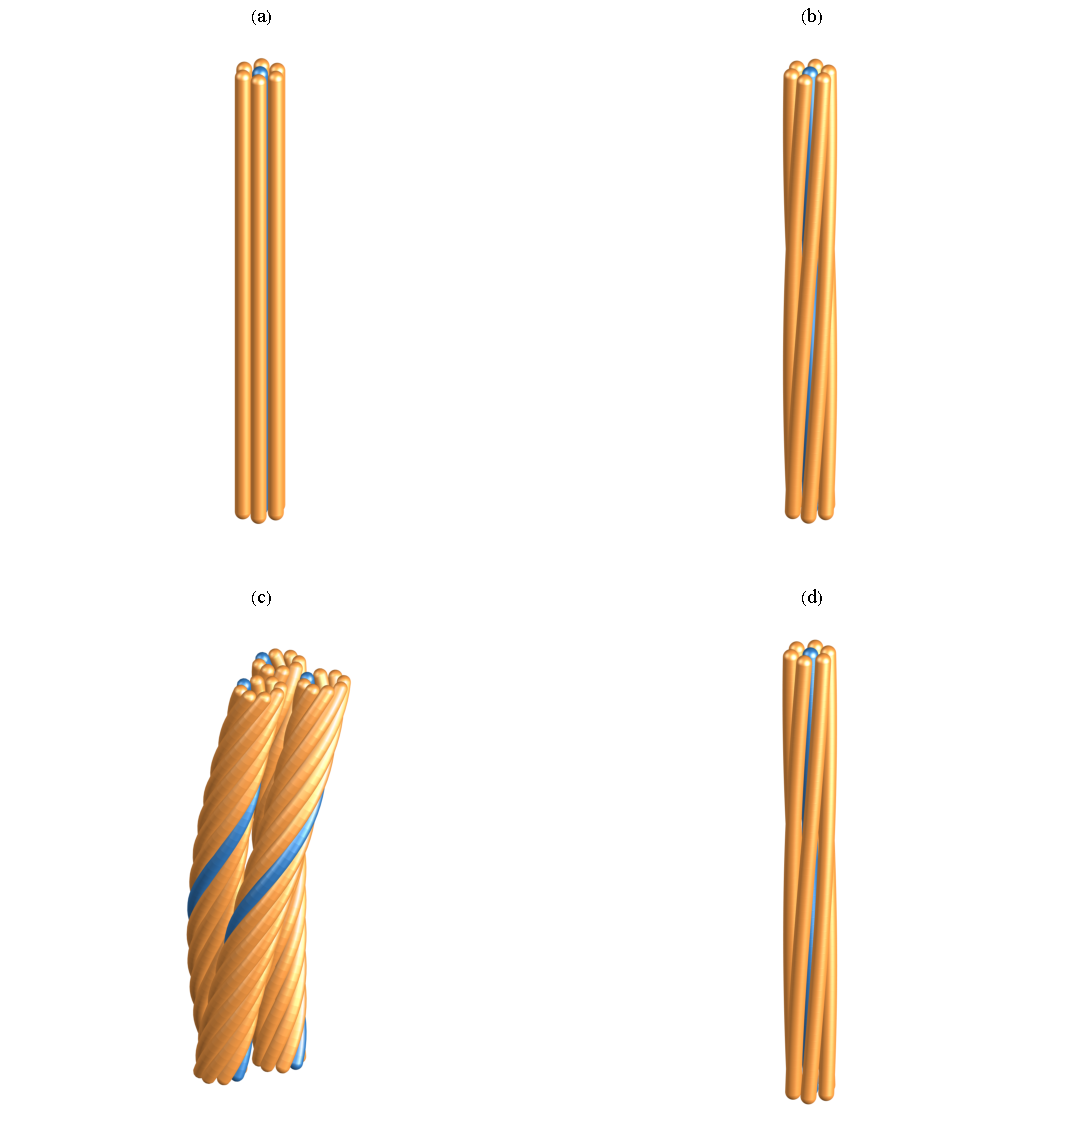
\includegraphics[width=\linewidth,height=.72\textheight,keepaspectratio]{../../assets/en/geometry_comparison.pdf}
\caption{Three-dimensional strand centerline structures. Panels show straight, single-level, local multilevel, and cross-layer structures. The 24-strand structures use a copper diameter of 0.100 mm, and the multilevel panel shows a 3 mm detail. Blue markers preserve selected physical strand identities.}
\label{fig:geometry_comparison}
\end{figure}
